\documentclass[a4paper]{article}

\usepackage[lmargin=25mm,rmargin=25mm,tmargin=25mm,bmargin=25mm]{geometry}
\usepackage{amsmath, amssymb}
\usepackage{babel}
\usepackage{hyperref}
\usepackage{xcolor}
\usepackage{graphicx}

\title{RoboCup 2024 \\ Standard Platform League (SPL) \\ Technical Challenge \\ --- \textsc{Shared Autonomy} --- \\\vspace{2cm} 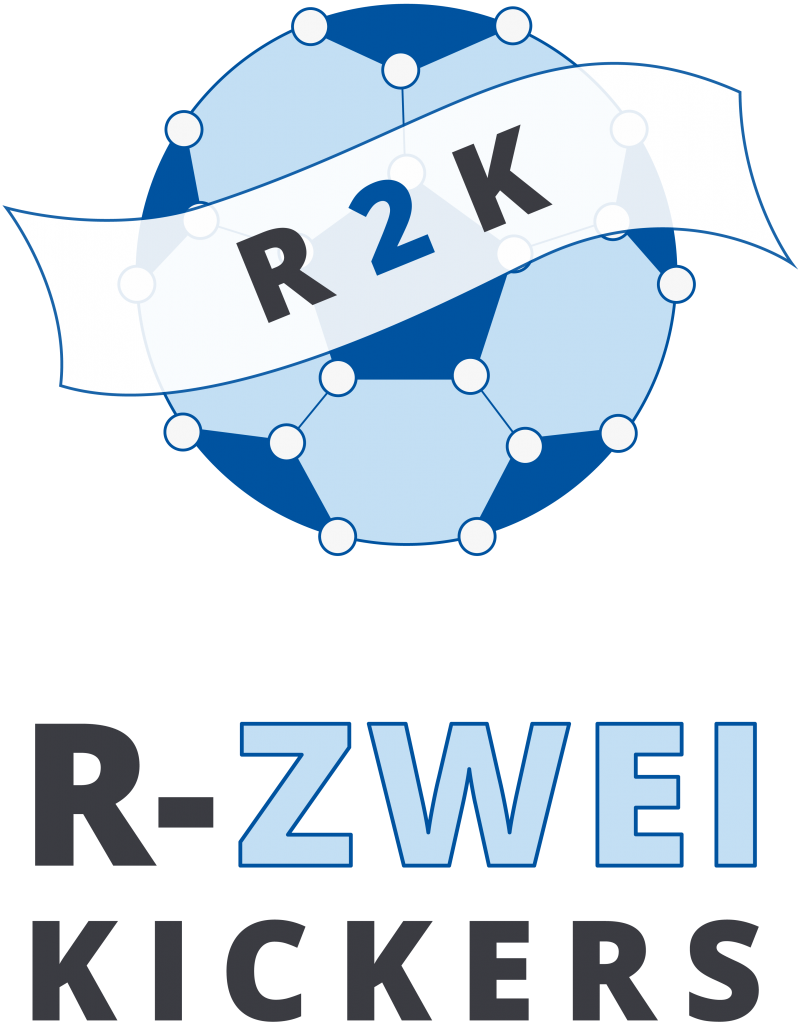
\includegraphics[width=0.5\textwidth]{img/R2K_Logo}}
\date{last updated: \today}
\author{Adrian Müller \\ Desmond Krämer \\ Samuel Njike Megaptche \\ Thomas Jäger \\ Wilhelm Simus}

\begin{document}
	\setlength{\parindent}{0pt}
	\pagestyle{empty}
	\maketitle
	\newpage
	%\tableofcontents
	\pagestyle{headings}

\section{The Challenge 2024: Shared Autonomy}

In the 2024 technical challenge, teams must create a mixed team comprising one human-operated Nao robot and one 
fully autonomous Nao robot. Matches will be played in a two vs. two format on the standard SPL field.

\subsection{The Goal}

The challenge aims to progress towards enabling robots to operate alongside agents with human-level intelligence. 
To ensure a level playing field in terms of physical capabilities, all participants will use Nao robots. 
Each team will have one robot remotely operated by a human, providing human-level intelligence, 
while the other robot will function autonomously, adhering to the main SPL competition rules.

For further references and exact rules, see 
\href{https://spl.robocup.org/wp-content/uploads/SPL-Challenges-2024.pdf}{\textcolor{blue}{the official challenge rules}} 
provided by the technical committee.

\section{Our Approach}

Our approach involves developing a sophisticated web-based interface to control the robots and facilitate communication. 
The backend system communicates with the robots via TCP, sending byte commands that are interpreted and 
executed by the robots.

\vspace{0.75cm}

\begin{figure}[h]
\centering
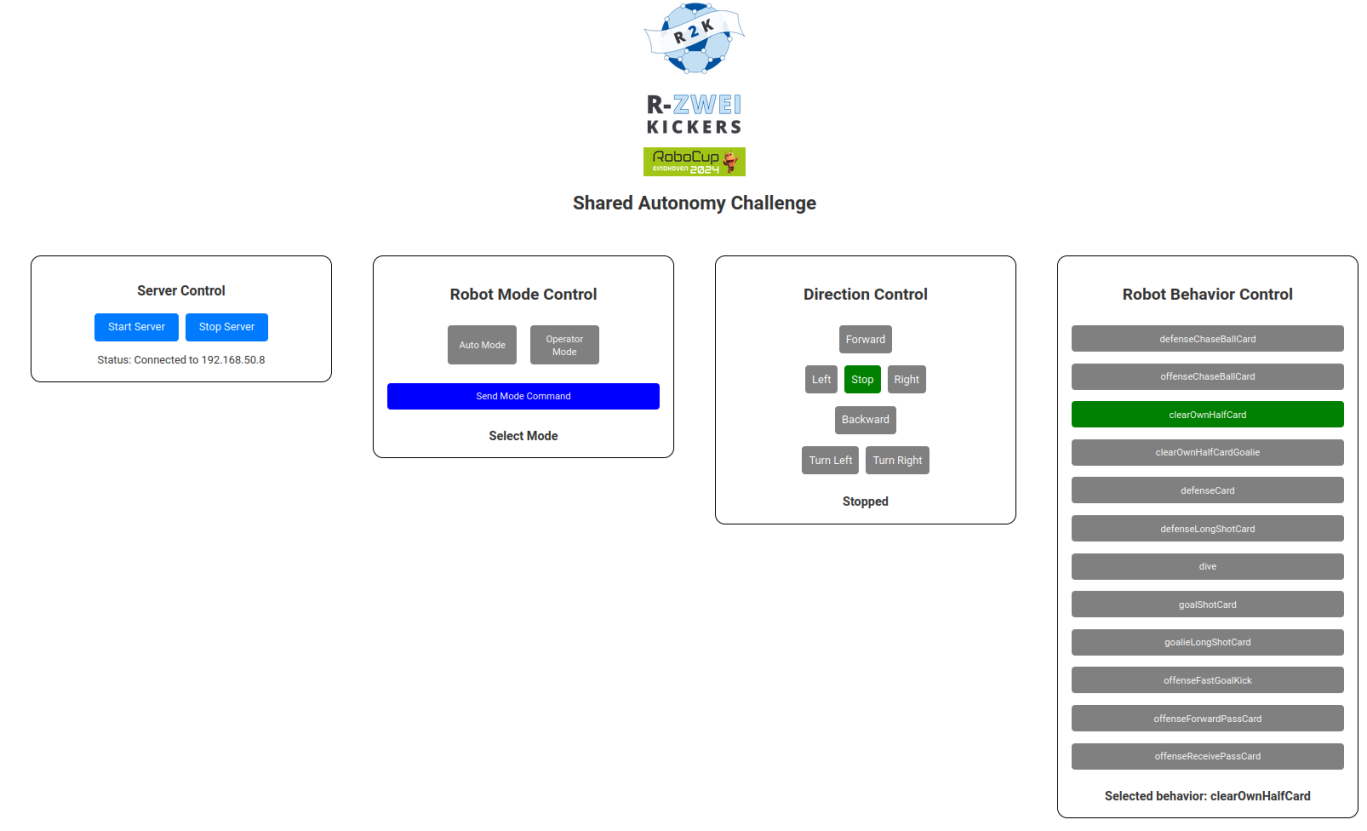
\includegraphics[width=\textwidth]{img/SAC}
\caption{The Interface for the shared autonomy challenge consists of four distinct control modules.}
\end{figure}

\subsection{Tactical Overview}

The interface is divided into several control modules:
- **Robot Mode Control**: This module allows switching between autonomous operation and full human control.
- **Direction Control**: Provides an interface for complete human control over the robot's movements.
- **Behavior Control**: Enables manual selection of behaviors from a prepared card stack using the BHuman skills and cards framework.

\newpage
\subsection{Technical Overview}

Our system is based on a minimalist web-app using Svelte for the frontend and a Python Flask server for the backend. The server acts as a REST interface, converting commands from the frontend to byte messages sent to the robot. The robot-side module interprets these messages, integrating the commands into its representation for use by other modules and parameterizing skills or behaviors.

\section{Future Enhancements}

To further enhance our system, we plan to improve inter-robot communication by enabling message exchanges between robots. 
Additionally, we aim to refine our tactical capabilities, offering more sophisticated and nuanced control options. \\

\textbf{Roadmap}

\begin{enumerate}
    \item \textbf{Inter-Robot Communication}: Implement triggers for message exchanges between robots to coordinate actions and strategies.
    \item \textbf{Enhanced Tactics}: Develop advanced tactical views and strategies to optimize robot performance in various scenarios.
    \item \textbf{User Interface Improvements}: Enhance the web interface to provide more intuitive and user-friendly controls.
\end{enumerate}

\end{document}
	
	
\end{document}